%MIT License
%
%Copyright (c) 2017 dinkoosmankovic
%
%Permission is hereby granted, free of charge, to any person obtaining a copy
%of this software and associated documentation files (the "Software"), to deal
%in the Software without restriction, including without limitation the rights
%to use, copy, modify, merge, publish, distribute, sublicense, and/or sell
%copies of the Software, and to permit persons to whom the Software is
%furnished to do so, subject to the following conditions:
%
%The above copyright notice and this permission notice shall be included in all
%copies or substantial portions of the Software.
%
%THE SOFTWARE IS PROVIDED "AS IS", WITHOUT WARRANTY OF ANY KIND, EXPRESS OR
%IMPLIED, INCLUDING BUT NOT LIMITED TO THE WARRANTIES OF MERCHANTABILITY,
%FITNESS FOR A PARTICULAR PURPOSE AND NONINFRINGEMENT. IN NO EVENT SHALL THE
%AUTHORS OR COPYRIGHT HOLDERS BE LIABLE FOR ANY CLAIM, DAMAGES OR OTHER
%LIABILITY, WHETHER IN AN ACTION OF CONTRACT, TORT OR OTHERWISE, ARISING FROM,
%OUT OF OR IN CONNECTION WITH THE SOFTWARE OR THE USE OR OTHER DEALINGS IN THE
%SOFTWARE.


    \documentclass[12pt]{article}
    \usepackage{amsfonts,amsmath,amssymb}
    \usepackage{amsmath,multicol,eso-pic}
    \usepackage[utf8]{inputenc}
    \usepackage[T1]{fontenc}
    \usepackage[left=2.00cm, right=2.00cm, top=2.00cm, bottom=2.00cm]{geometry}
    \usepackage{titlesec}
    \usepackage{enumerate}
    \usepackage{multirow}
    \usepackage{listings}
    \usepackage{breqn}
    \usepackage{tikz}
     \usetikzlibrary{automata, positioning}
    \usepackage{rotating}
     \usepackage{pgfplots}
    \usepackage{colortbl}
    \usepackage{xcolor}
    %\renewcommand{\wedge}{~}
    %\renewcommand{\neg}{\overline}
    \titleformat{\section}{\large}{\thesection.}{1em}{}
    
    
    % % % % % POPUNITE PODATKE
    
    \newcommand{\prezimeIme}{Hamzić Huso}
    \newcommand{\brIndexa}{18305}
    \newcommand{\brZadace}{5}
    \newcommand{\grupa}{DM2 Pon[15.00]}
    \newcommand{\demos}{Šeila Bećirović}
    % % % % % 
    
    \begin{document}
    
    \thispagestyle{empty}
    \begin{center}
      \vspace*{1cm}

      \vspace*{2cm}
      {\huge \bf Zadaća \brZadace } \\
      \vspace*{1cm}
      {\Large \bf iz predmeta Diskretna matematika}

      \vspace*{2cm}

      {\Large Prezime i ime: \prezimeIme} \\
      \vspace*{0.75cm}
      {\Large Broj indeksa: \brIndexa} \\
      \vspace*{0.75cm}
      {\Large Grupa: \grupa} \\
      \vspace*{0.75cm}
      {\Large Odgovorni asistent: \demos} \\
      \vspace*{2cm}
      \renewcommand{\arraystretch}{1.75}
      \vfill


      {\large Elektrotehnički fakultet Sarajevo}

    \end{center}
    \newpage
    \thispagestyle{empty}
    
    
    % % % % % Rješenja zadataka
	\begin{enumerate}
	\item Dat je periodični diskretni signal perioda 6, čije vrijednosti u trenucima 0, 1, 2, 3, 4 i 5 respektivno iznose 2, 9, –7, –7, –5 i –9.\\
a) Predstavite ovaj diskretni signal formulom u kojoj se javlja cijeli dio broja;\\
b) Predstavite ovaj signal diskretnim Fourierovim redom;\\
c) Odredite amplitudni i fazni spektar za ovaj signal i predstavite ga u vidu sume harmonika.\\
\begin{center}
    \textit{a) Svaki periodični signal osnovnog perioda N se može izraziti kao suma N članova u kojima figurira funkcija "cijeli dio broja":\\
$x_n = x_{-1} + \sum^{N-1}_{k=0} (x_k - x_{k-1}) \lfloor\frac{n-k}{N}\rfloor$}\\
Poznate su nam vrijednosti $x_n$ za N[0..5] pa uvrštavanjem imamo:\\
\underline{$x_n = -9 + 11\cdot \lfloor\frac{n}{6}\rfloor + 7 \cdot \lfloor\frac{n-1}{6}\rfloor -16 \cdot \lfloor\frac{n-2}{6}\rfloor + 0 \cdot \lfloor\frac{n-3}{6}\rfloor + 2 \cdot \lfloor\frac{n-4}{6}\rfloor - 4 \cdot \lfloor\frac{n-5}{6}\rfloor$}\\
\vspace{0.25cm}
\textit{b) Svaki periodični diskretni signal se može izraziti kao suma konačno mnogo harmonijskih diskretnih signala. Oblik diskretnog Fourierovog reda:\\
\begin{equation*}
		    x_n = \frac{a_0}{2} + \sum_{k = 1}^{\lfloor~N/2~\rfloor} a_k~cos\frac{2k\pi}{N}n + b_k~sin\frac{2k\pi}{N}n
		\end{equation*}
		\begin{equation*}
		    a_k = \frac{2}{N}~\sum_{n = 0}^{N - 1} x_n~cos\frac{2k\pi}{N}n, ~ k = 0,1,...,\lfloor~\frac{N}{2}~\rfloor
		\end{equation*}
		\begin{equation*}
		    b_k = \frac{2}{N}~\sum_{n = 0}^{N - 1} x_n~sin\frac{2k\pi}{N}n, ~ k = 0,1,...,\lfloor~\frac{N}{2}~\rfloor
		\end{equation*}\\
Treba napomenuti da se kod računanja $a_k$ za k=N/2 ispred sume javlja 1/N (umjesto 2/N) kada je N paran broj.	\\ Računanjem dobijamo sljedeće koeficijente:\\	
\fbox{$a_{0} = -17/3$} 
\fbox{$a_{1} = 5$} 
\fbox{$a_{2} = 1/3$}
\fbox{$a_{3} = 1/2$} \\
\fbox{$b_{1} =-\sqrt{3}/3$} 
\fbox{$b_{2} = 10\cdot\sqrt{3}/3$} 
\fbox{$b_{3} = 0$} \\
\vspace{0.25cm}
Pa je naš diskretni Fourierov red:\\
\underline{$x_n = -\frac{17}{6} + 5 \cdot cos \frac{n\pi}{3} - \frac{\sqrt{3}}{3} \cdot sin \frac{\pi}{3}n + \frac{1}{3} \cdot cos\frac{2\pi}{3}n + 10\frac{\sqrt{3}}{3} \cdot sin\frac{2\pi}{3}n + \frac{1}{2}\cdot cos(n\pi)$}\\
\vspace{0.25cm}
c) Odredimo amplitudni i fazni spektar signala:\\
 \begin{equation*}
		    x_n = \sum_{k = 0}^{\lfloor~N/2~\rfloor} A_k~sin(\frac{2k\pi}{N}n + \varphi_k) ~(*)
		\end{equation*}
		\begin{equation*}
		    A_k = \sqrt{a_k^2 + b_k^2} \quad \varphi_k = arctg\frac{a_k}{b_k}
		\end{equation*}
Iz čega slijedi:\\
\fbox{$A_0 = -17/3$}
\fbox{$A_1 = 2\sqrt{57}/3$}
\fbox{$A_2 = \sqrt{301}/3$}
\fbox{$A_3 = 1/2$}\\
\fbox{$ \phi_{0} = -\pi/2$}
\fbox{$ \phi_{1} = arctg (\frac{-15}{\sqrt{3}})$}
\fbox{$ \phi_{2} = arctg(\frac{1}{10\sqrt{3}})$}
\fbox{$ \phi_{3} = \pi/2$}\\
Nakon što raspišemo izraz za $x_n$ sa dobijenim vrijednostima, imamo:\\
\underline{$x_n = -\frac{17}{3} + 2\frac{\sqrt{57}}{3}\cdot cos (\frac{\pi}{3}n + arctg (\frac{-15}{\sqrt{3}})) +  \frac{\sqrt{301}}{3} \cdot cos(\frac{2\pi}{3}n +  arctg(\frac{1}{10\sqrt{3}})) + \frac{1}{2}cos(n\pi + \frac{\pi}{2})$}
}
\end{center}

	\item Ispitajte koji su od sljedećih diskretnih signala periodični a koji nisu. Za one koji jesu, nađite osnovni period N:\\
a) $sin (2n\pi/15) + 3 cos (5n\pi/21 + \pi/4)$\\
b) $sin (3n\pi/4) cos (2n\pi/5)$\\
c) $(n + 1) cos (n\pi/5)$ – $ncos(9n\pi/5)$\\
d) ${(-1)}^{n} cos (4n\pi/7)$\\
Odgovori moraju biti obrazloženi, inače se neće priznavati!\\
\begin{center}
    \textit{a) f = $sin (2n\pi/15) + 3 cos (5n\pi/21 + \pi/4)$\\Najprije ćemo rastaviti funkciju na prvi i drugi dio:\\$f_1(x) = sin (2n\pi/15)$ i $f_2(x) =  3 cos (5n\pi/21 + \pi/4)$\\
    Period prvog dijela je očigledno 15, obzirom da se po formuli $T = \frac{2\pi}{w}$ lako dobije da je w = 15, pa je i \fbox{$T_1 = 15$}.\\Što se tiče drugog dijela funkcije, računanje perioda je nešto složenije. Prije svega moramo shvatiti da $\frac{\pi}{4}$ nema utjecaja na period funkcije obzirom da ne ovisi od n i njen period je 0.\\Ostaje nam prvi dio $f_2$, odnosno $sin(3 cos (\frac{5n\pi}{21}))$ čiji je period jednak T = $\frac{2\pi}{\frac{5\pi}{21}}$, odnosno \fbox{$T_2 = \frac{42}{5}$}. Ono što preostaje jeste da nađemo najmanji zajednički sadržilac za vrijednosti perioda iz dva dijela naše funkcije, tj. NZS (42, 15) = 210, što je i period naše funkcije T.\\ \fbox{$T_f = 210$}\\
    \vspace{0.5cm}
    b) Primijetimo da je f sastavljena od $f_1 = sin(3n\pi/4)$ i $f_2=cos(2n\pi/5)$ odakle očito imamo da je period $T_1 = \frac{2\pi}{\frac{3\pi}{4}}$ odnosno imamo da je $T_1$ = 8/3\\
    analogno imamo da je $T_2$ = 5 pa je onda period funkcije f $NZS(\frac{8}{3},\frac{1}{5})$ odnosno \fbox{T=40}\\
    \vspace{0.3cm}
   c) f(n)=$(n + 1) cos (n\pi/5)$ – $ncos(9n\pi/5) = n[cos(\frac{n\pi}{5}) - cos(\frac{9n\pi}{5})] + cos(\frac{n\pi}{5}) = -2n\cdot sin\frac{\frac{n\pi}{5} + \frac{9n\pi}{5}}{2}sin\frac{\frac{n\pi}{5} - \frac{9n\pi}{5}}{2} +  cos(\frac{n\pi}{5}) = 
   2n\cdot sin(n\pi) sin(\frac{4n\pi}{5}) +  cos(\frac{n\pi}{5})$\\
   \vspace{0.3cm} 
   Odakle se jasno vidi da je za $n\in N$ ili $n\in Z$, f(n) = $cos(\frac{n\pi}{5})$ odnosno
   $\Omega = \frac{\pi}{5}$, p = 1, q = 5 pa je onda \fbox{T = 2q = 10}\\
   \vspace{0.5cm}
   d)  f(n) = ${(-1)}^{n} cos (4n\pi/7) = cos(n\pi)cos(\frac{4n\pi}{7}) = \frac{1}{2}[cos(n\pi - \frac{4n\pi}{7}) + cos(n\pi + \frac{4n\pi}{7})]$ \\ \vspace{0.3cm} =$\frac{1}{2}[cos(\frac{3n\pi}{7}) + cos(\frac{9n\pi}{7})]$\\
   \vspace{0.3cm}
   odakle jasno vidimo da 1/2 ne igra ulogu na period već da će samo periodi ovih kosinusa igrat ulogu u periodu početne funkcije, analogno prethodnim zadacima odmah vidimo da je period prvog kosinusa $T_1 = \frac{14}{3}$ a period drugog $T_2 = \frac{14}{9}$ odakle imamo da je period početne funkcije\\ \fbox{T = $NZS(T_1, T_2) = 14$}}
\end{center}
	\item Odredite i nacrtajte amplitudno-frekventnu i fazno-frekventnu karakteristiku diskretnog sistema opisanog diferentnom jednačinom $y_n - 9y_{n-1} = 2x_n - 7 x_{n-1}$, a nakon toga, odredite odziv ovog sistema na periodični signal iz Zadatka 1. Uputa: razmotrite prolazak svakog od harmonika posebno.
	\begin{center}
	\newpage
	     \textit{Nađimo prvo funkciju sistema H(z). Ako izvršimo Z transformaciju lijeve i desne strane, naša diferentna jednačina postaje: $ z^n H(z) - 9 z^{n-1} H(z) = 2 z^n - 7 z^{n-1}$\\Odavde je H(z) = $\frac{2z^2 - 7z}{z^2 - 9z}$\\
	     \vspace{0.3cm}
	    Amplitudno-frekventnu karakteristiku nalazimo kao:\\ A($\Omega$) = |H$e^{i\Omega}$|.}\\
	    A($\Omega$) = |$\frac{2 e^{2i\Omega} - 7 e^{i\Omega}}{e^{2i\Omega} - 9 e^{i\Omega}}$| = |$\frac{-7 + 2 e^{i\Omega}}{-9 + e^{i\Omega}}$| = |$\frac{-7 + 2 (cos \Omega + i \cdot sin \Omega)}{-9 + (cos \Omega + i \cdot sin \Omega)}$| = $\sqrt{\frac{(-7 + 2 cos \Omega)^2 + 4 sin^2 \Omega}{(-9 + cos \Omega)^2 + sin^2 \Omega}}$=\\
	     = $\sqrt{\frac{53 - 28 cos \Omega}{82 - 18 cos \Omega}}$\\
	    \vspace{0.25cm}
	    Obzirom da je A($\Omega$) periodična funkcija, dovoljno ju je skicirati na intervalu [-$\pi$, $\pi$]:\\
	    \vspace{0.3cm}
	    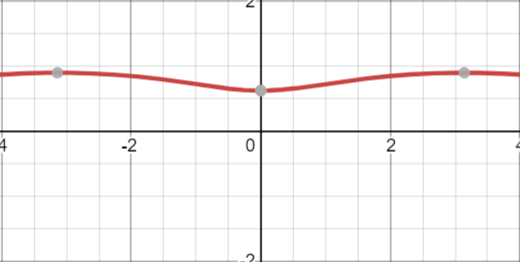
\includegraphics[width=120mm]{grafA.png}\\
        \vspace{0.5cm}
	    Nađimo sada fazno-frekventnu karakteristiku $\Phi(\omega)$:\\
	    $\Phi(\Omega)$ = arg($\frac{-7 + 2 \cdot cos \Omega + 2 \cdot i \cdot sin \Omega}{-9 + cos \Omega + i \cdot sin \Omega)}$) = \\
	    .\\.\\. \\Nema se profesore kada raspisivati, ispitna sedmica :(\\
	    \vspace{0.3cm}
	    = arg[$\frac{65 - 25cos\Omega}{{(cos\Omega - 9)}^{2} + {sin}{2}\Omega} + i \cdot \frac{ - 14  \cdot sin(\Omega) \cdot cos(\Omega) + 19  \cdot sin(\Omega)}{10 - 6 cos \Omega}$]\\
	    Vrijedi
	    $\Phi(\Omega)$ = $-\pi + arctg(\frac{Im(z)}{Re(z)}) = -\pi + arctg (\frac{-11sin\Omega}{65 - 25cos\Omega})$\\
	    \vspace{0.25cm}
	    Skicirajmo i grafik  $\Phi(\Omega)$:\\
	     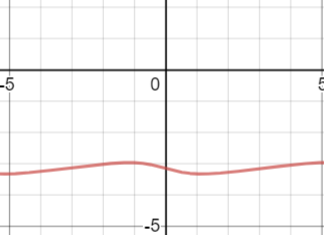
\includegraphics[width=120mm]{grafFi.png}\\
	    \vspace{0.25cm}
	    Preostaje nam još samo da odredimo odziv sistema na periodični signal iz prvog zadatka:\\
	    $y_n = 2 x_n - 7 x_{n-1} + 9y_{n-1}$.\\Obzirom da je sistem kauzalan (ne ovisi od budućih vrijednosti $x_n$), tj. iz $x_n$=0 za n<0 slijedi $y_n$=0 za n<0, imamo:\\
	    $y_0 = 2 x_0 - 7 x_{-1} + 9y_{-1}$\\
	    $y_1 = 2 x_1 - 7 x_{0} + 9y_{0}$\\
	    $y_2 = 2 x_2 - 7 x_{1} + 9y_{1}$\\
	    $y_3 = 2 x_3 - 7 x_{2} + 9y_{2}$\\
	    \vspace{0.25cm}
	    Sada ćemo razmotriti prolazak svakog od harmonika iz prvog zadatka posebno:\\
	    \underline{1. $x_n =\frac{-17}{3}$} \\
	    \vspace{0.25cm}
	    Prateći gore izvedene relacije dobijamo redom:\\
	      $y_0 = \frac{-34}{3}$\\ \vspace{0.3cm}
	    $y_1 = \frac{-221}{3}$ \\\vspace{0.3cm}
	    $y_2 =\frac{-1904}{3}$\\\vspace{0.3cm}
	    $y_3 = \frac{-17051}{3}$\\\vspace{0.3cm}
	     \vspace{0.25cm}
	     \underline{2. $x_n =\frac{\sqrt{301}}{3} \cdot cos(\frac{2\pi}{3}n +  arctg(\frac{1}{10\sqrt{3}}))$}\\
	     \vspace{0.25cm}
	        $y_0 = 20\frac{\sqrt{3}}{3}$\\
	    $y_1 = 33\sqrt{3}$\\
	    $y_2 = 1841\frac{\sqrt{3}}{6}$\\
	    $y_3 = 8836\frac{\sqrt{3}}{3}$\\
	      \newpage
	     \underline{3. $x_n =  2\frac{\sqrt{57}}{3}\cdot cos (\frac{\pi}{3}n + arctg (\frac{-15}{\sqrt{3}}))$}\\
	     \vspace{0.25cm}
	        $y_0 = 2\frac{\sqrt{3}}{3}$ \\
	    $y_1 = 9\sqrt{3}$\\
	    $y_2 = 67\sqrt{3}$\\
	    $y_3 = 586\sqrt{3}$\\
	      \vspace{0.25cm}
	     \underline{4. $x_n = \frac{1}{2} \cdot cos (\pi n + \frac{\pi}{2})$}\\
	     \vspace{0.25cm}
	        $y_0 = 0$\\
	    $y_1 = 0$\\
	    $y_2 = 0$\\
	    $y_3 = 0$\\
	      \vspace{0.25cm}
	\end{center}
	\item Nađite z-transformaciju sekvence $x_n = (n^2 cos (\frac{n\pi}{3}) + \frac{(5)^n}{(2n + 1)!} ) u_{n-2}$. Pri tome se po potrebi možete koristiti tablicama i osobinama z-transformacije.\\
	\begin{center}
    Na početku riješimo sve prvo osim $u_{n-2}$ odnosno ovo u zagradi. Prvi dio ovog u zagradi je oblika $n^ky_{1n}$ (gdje je $y_{1n}$ samo oznaka). Prvo nađimo Z transformaciju kosinusa koju iščitavamo iz tablice:\\
    $Y_1(z) = \frac{2z^2 - z}{2z^2 - 2z + 2}$.\\
    Zatim drugo pravilo kaže za transformaciju sekvenci oblika $n^ky_1n$ imamo :\\
    $X_1(z) = (-z\frac{d}{dz})^2Y_1(z) = -z\frac{d}{dz}[-z\frac{d}{dz}(\frac{2z^2 - z}{2z^2 - 2z + 2})] = \frac{z^5 + 7z^4 + 7z^2 - z}{2(z^2-z+1)^3}$ \\
    \vspace{0.3cm} 
    Sad je potrebno naći transformaciju drugog dijela naše osnovne sekvence odnosno $\frac{5^n}{(2n+1)!}$.\\
    Razdvojimo ovo na dvije sekvence pa imamo da je $Z\{ \frac{1}{(2n+1)!} \} = \frac{\sqrt{z}}{2}[e^{\frac{1}{\sqrt{3}}} - e^{\frac{-1}{\sqrt{3}}}]$ \\
    \vspace{0.3cm} 
    Sada na osnovu pravila o Z transformaciji sekvence pomnožene sa $a^n$ slijedi da je \\
     $Z\{ \frac{5^n}{(2n+1)!} \} = \frac{\sqrt{z}}{2\sqrt{5}}[e^{\frac{\sqrt{5}}{\sqrt{3}}} - e^{\frac{-\sqrt{5}}{\sqrt{3}}}]$ \\
     \vspace{0.3cm}
     Pa imamo konačno uzevši u obzir u $u_{n-2}$ da je naše Y(z) :
     $Y(z) = \frac{z^5 + 7z^4 + 7z^2 - z}{2(z^2-z+1)^3} + \frac{\sqrt{z}}{2\sqrt{5}}[e^{\frac{\sqrt{5}}{\sqrt{3}}} - e^{\frac{-\sqrt{5}}{\sqrt{3}}}] - 1 - \frac{4}{3z}$
   
	\end{center}
	\item Dat je diskretni sistem opisan diferentnom jednačinom $7y_{n+3} + 5 y_{n+2} = 3 x_{n+3}-2x_n$. Nađite odziv ovog sistema na pobudu $x_n = n sin (7n \pi / 4) u_n$. Rješenje treba izraziti u obliku u kojem se ne javljaju kompleksni brojevi.\\
	\begin{center}
	   
	    Ako stavimo da je $x_n = z^n$ i $y_n = z^nH(z)$ imamo:\\
	    $7z^{n+3}H(z) + 5z^{n+2}H(z) = 3z^{n+3} -2z^n$ odnosno \\
	    \vspace{0.3cm}
	   \fbox{$H(z) = \frac{3z^3-2}{7z^3+5z^2}$}\\
	   
	   Nađimo sada X(z) kao X(z) = $-z\frac{d}{dz}[Z\{sin\frac{7n\pi}{4}\}]$ odnosno očitavajući iz tablica Z transformaciju sinusa i diferencirajući po z dobijamo: \\
	   \vspace{0.3cm}
	   X(z) = $\frac{z-z^3}{\sqrt{2}(z^2-\sqrt{2}z+1)^2}$\\
	   a kako vrijedi da je Y(z)=X(z)H(z) dobijamo da je: \\
	   \vspace{0.3cm}
	   
	   Y(z) = $\frac{-(z^2-1)(3z^2-2)}{z\sqrt{2}(7z+5)(z^2-\sqrt{2}z+1)^2}$
	   \\
	   nule karakterističnog polinoma su z=0, $z=\frac{-5}{7}$, $z=\frac{1-i}{\sqrt{2}}$,  $z=\frac{1+i}{\sqrt{2}}$ gdje su ove dvije zadnje višestruke pa inverznu Z transformaciju ćemo naći uz pomoć rezidiuma jer se 
	   $y_n$ može napisati kao: \\
	   \vspace{0.3cm}
	   $y_n =[Res(Y(z)z^{n-1})]_{z=0} + [Res(Y(z)z^{n-1})]_{z=\frac{-5}{z}} 
	   + [Res(Y(z)z^{n-1})]_{z=\frac{1+i}{\sqrt{2}}} + [Res(Y(z)z^{n-1})]_{z=\frac{1-i}{\sqrt{2}}}$ \\
 
        \vspace{0.3cm}
        Gdje se prva dva rezidiuma računaju lagano kao: \\
        \vspace{0.3cm}
        $[Res(Y(z)z^{n-1})]_{z=0} = \lim_{z \to 0} [\frac{-(z^2-1)(3z^2-2)z z^{n-1}}{z\sqrt{2}(7z+5)(z^2-\sqrt{2}z+1)^2}] = \frac{-\sqrt{2}}{5}\delta_{n-1}$ \\
        \vspace{0.3cm}
        Analogno dobijamo i drugi rezidium iznosi $\frac{6366\sqrt{2}}{35(3963+2590\sqrt{2})}(\frac{-5}{7})^{n-1}$
        \\
        \vspace{0.3cm}
        Treći rezidium ćemo računati kao: \\
        \vspace{0.3cm}
        $[\frac{d}{dz}\{ \frac{-(z^2-\sqrt{2}z+1)z^{n-1}(z^2-1)(3z^2-2)}{z\sqrt{2}(7z+5)(z^2-\sqrt{2}z+1)^2}} \}]_{z=\frac{1+i}{\sqrt{2}}}$ \\
        \vspace{0.25cm}
        gdje nakon malo dužeg računa dobijamo da on iznosi: \\
        \vspace{0.3cm}
        $(\frac{1-i}{\sqrt{2}})^n \frac{(\frac{1}{2} + \frac{i}{2})[(5i-1)(n-1) - (11+i)\sqrt{2}]}{\sqrt{2}(5+\frac{7-7i}{\sqrt{2}})^2}$
        \\
        \vspace{0.3cm}
        analogno četvrti iznosi: \\
        \vspace{0.3cm}
        $(\frac{1+i}{\sqrt{2}})^n \frac{(\frac{1}{2} - \frac{i}{2})[(-5i-1)(n-1) - (11-i)\sqrt{2}]}{\sqrt{2}(5+\frac{7-7i}{\sqrt{2}})^2}$
        \\
        \vspace{0.3cm}
        Pa je onda naše $y_n$\\
        \vspace{0.3cm}
        $y_n = \frac{-\sqrt{2}}{5}\delta_{n-1} + \frac{6366\sqrt{2}}{35(3963+2590\sqrt{2})}(\frac{-5}{7})^{n-1} + (\frac{1-i}{\sqrt{2}})^n \frac{(\frac{1}{2} + \frac{i}{2})[(5i-1)(n-1) - (11+i)\sqrt{2}]}{\sqrt{2}(5+\frac{7-7i}{\sqrt{2}})^2} + + (\frac{1+i}{\sqrt{2}})^n \frac{(\frac{1}{2} - \frac{i}{2})[(-5i-1)(n-1) - (11-i)\sqrt{2}]}{\sqrt{2}(5+\frac{7-7i}{\sqrt{2}})^2}$
        
        
	\end{center}
    \end{enumerate}

    \end{document}
    